% =====================================================================
% TmFeO3 2DCS — Supplemental Material
% Condensed from tmfeo3_foundation.tex (full derivations there)
% =====================================================================
\documentclass[11pt]{article}
\usepackage{amsmath,amssymb,mathtools,bm}
\usepackage{graphicx}
\usepackage{geometry}
\geometry{margin=2.4cm}
\usepackage{booktabs,array}
\usepackage{xcolor}
\usepackage{hyperref}
\hypersetup{colorlinks=true,linkcolor=blue,citecolor=blue,urlcolor=blue}
\usepackage{cleveref}

\newcommand{\Fe}{\mathrm{Fe}}
\newcommand{\Tm}{\mathrm{Tm}}
\newcommand{\diag}{\mathrm{diag}}
\newcommand{\ket}[1]{|#1\rangle}
\newcommand{\bra}[1]{\langle #1|}
\newcommand{\ve}[1]{\boldsymbol{#1}}
\newcommand{\qafm}{q_{\rm AFM}}
\newcommand{\qfm}{q_{\rm FM}}
\newcommand{\Mnl}{M_{\rm NL}}
\renewcommand{\thesection}{S\arabic{section}}
\renewcommand{\thetable}{S\arabic{table}}
\renewcommand{\thefigure}{S\arabic{figure}}

\title{Supplemental Material for\\
``Magnon--crystal-field cross peaks in two-dimensional terahertz
spectroscopy of TmFeO$_3$''}
\author{}
\date{\today}

\begin{document}
\maketitle
\tableofcontents

% =====================================================================
\section{The SU(3) qutrit and why its classical dynamics is quantum-exact}
\label{si:qutrit}
% =====================================================================

Tm$^{3+}$ is $4f^{12}$, $^3H_6$ ($J=6$).  In the $C_s(m)$ crystal field of
the $Pbnm$ $4c$ site the 13-fold multiplet splits into 13 singlets; the
model keeps the three lowest, $\ket{1},\ket{2},\ket{3}$, with splittings
$E_{12}=2.068$\,meV ($0.50$\,THz) and $E_{13}=4.963$\,meV ($1.20$\,THz),
consistent with the measured lines $E_{12}+E_{23}\approx E_{13}$.  The
site state is the Gell-Mann vector $\lambda^a=\mathrm{Tr}(\rho\Lambda^a)$,
$a=1\dots8$, and every single-ion term (CEF energies, external drives,
exchange mean fields) is \emph{linear} in the $\Lambda^a$.  For a
Hamiltonian linear in the generators the von Neumann equation
$\dot\rho=-i[H,\rho]$ closes on $\vec\lambda$:
\begin{equation}
  \dot\lambda^a \;=\; \Omega_{ab}(t)\,\lambda^b
  -\gamma_a\big(\lambda^a-\lambda^a_{\rm eq}\big),\qquad
  \Omega_{ab}=\tfrac12\,\mathrm{Tr}\!\left(\Lambda^a\,
  (-i)[H(t),\Lambda^b]\right).
\end{equation}
The classical SU(3) propagation is therefore the \emph{exact} quantum
dynamics of the driven, damped three-level ion, and a Boltzmann-weighted
ensemble of trajectories launched from the level seeds
$\ket1,\ket2,\ket3$ is the exact thermal density matrix for single-ion
drives.  (This was verified explicitly against an independent
density-matrix integrator; the two censuses agree to all digits quoted.)
Damping is Bloch-type on the Gell-Mann pairs of each transition,
$\gamma(\lambda^{1,2}),\gamma(\lambda^{4,5}),\gamma(\lambda^{6,7})$, with
population relaxation $\gamma(\lambda^{3,8})$ toward the equilibrium
populations captured at initialization.

The magnetically bright coordinate of the $E_{12}$ block follows from the
projected moment $P J_z P=5.264\,\lambda^2$: only $\lambda^2$ radiates
magnetically, and the onsite splitting drives the planar precession
$\dot\lambda^1=-\Delta_{12}\lambda^2$,
$\dot\lambda^2=+\Delta_{12}\lambda^1$, so the $E_{12}$ sector is a single
driven oscillator
\begin{equation}
  \lambda^2(t)=\int_0^t \sin[\omega_{12}(t-t')]\,h^1(t')\,dt',
  \label{eq:si-osc}
\end{equation}
where $h^1$ is the effective force a conversion vertex exerts on
$\lambda^1$.  All delay-axis structure of a cross peak lives in the
$\tau$-dependence of $h^1$.

% =====================================================================
\section{Crystallography and the projected Fe--Tm coupling}
\label{si:crystal}
% =====================================================================

TmFeO$_3$ is $Pbnm$ ($Z=4$): Fe$^{3+}$ at $4b$ (site symmetry $\bar1$;
every Fe sits on an inversion center), Tm$^{3+}$ at $4c$ (site symmetry
the single mirror $m_z$).  Inversion maps each Fe sublattice to itself
and exchanges Tm sublattices in pairs; the local mirror is the physical
$4c$ site mirror and generates the relative $\lambda^5,\lambda^7$ signs
between Tm sublattices.  The Fe order is G-type
($T_N\approx632$\,K) with DM canting; below the spin reorientation
($T_2\approx85$\,K) the ground state is $\Gamma_2=(F_x,C_y,G_z)$.

The Fe--Tm sector is built from the physical operator route
\begin{equation}
  \ve S,\ \ve J\ \longrightarrow\ H_{\Fe-\Tm}=\ve S^TA\,\ve J
  \ \longrightarrow\ P\ve JP
  \ \longrightarrow\ \text{couplings to }\lambda^a ,
\end{equation}
never by assuming that a space-group rotation acts as a closed onsite
SU(3) rotation in one fixed qutrit basis.  Working in a
\emph{transported gauge} (qutrit bases on the four Tm sublattices related
by the group operations themselves) makes every bond formula explicit and
turns the irrep ($\Gamma_1$) projection into simple four-site sign sums.
Time-reversal splits the Gell-Mann set into
$\lambda^-=\{\lambda^2,\lambda^5,\lambda^7\}$ (odd) and
$\lambda^+=\{\lambda^1,\lambda^3,\lambda^4,\lambda^6,\lambda^8\}$ (even);
every coupling term must be $\mathcal T$-even overall, which fixes how
many Fe-spin or $B$-field legs may attach to each sector.  The candidate
couplings through cubic order in the fields are
\begin{center}
\renewcommand{\arraystretch}{1.25}
\begin{tabular}{llll}
\toprule
family & operator form & sector & legs \\
\midrule
$K^-$ & $S_\alpha\lambda^a$ & $\lambda^-$ & 1 Fe \\
$ESJ$ & $E_\eta S_\alpha\lambda^a$ & $\lambda^-$ & 1 E-photon + 1 Fe \\
$\kappa^B$ & $B_\eta S_\alpha\lambda^a$ & $\lambda^+$ & 1 B-photon + 1 Fe \\
$W$ & $S_\alpha S_\beta\lambda^a$ & $\lambda^+$ & 2 Fe \\
\bottomrule
\end{tabular}
\end{center}
The full orbit formulas (all eight coefficients per bond, all four Tm
sublattices, both time-reversal sectors) and the implementation
prescriptions for global-axis versus local-frame storage are given in the
long-form working note that accompanies the data
(\texttt{tmfeo3\_foundation.tex}, Secs.~3--14).

% =====================================================================
\section{The sharp requirement and the vertex scorecard}
\label{si:scorecard}
% =====================================================================

Two collinear pulses give $\Mnl=M_{AB}-M_A-M_B$; order by order only the
mixed terms survive, so $\Mnl$ starts at second order and the leading
robust magnetic-dipole contribution is third order.  Combining
Eq.~\eqref{eq:si-osc} with the conservation rules at each vertex (energy;
$\mathcal T$-parity; $\Gamma_1$) yields six requirements for a coupling
to produce the geometry-A cross peak at $(\qafm,E_{12})$:
\begin{description}
\item[R1 (detection)] reaches $\lambda^1/\lambda^2$ (the $E_{12}$ block);
\item[R2 (drive)] is sourced by the pumped $\delta S_y$ magnon;
\item[R3 (parity)] is $\mathcal T$-even (fixes the $\lambda^\pm$ sector);
\item[R4 (irrep)] is $\Gamma_1$-allowed in the $\Gamma_2$ state;
\item[R5 (energy)] carries the $0.90\to0.50$\,THz mismatch (needs $\geq2$
  non-$\lambda$ legs);
\item[R6 ($\Mnl$)] involves both pulses.
\end{description}

\begin{table}[h]
\centering\small
\caption{Vertex scorecard.  Only $W$ and $\kappa^B$ pass all six
requirements.}
\begin{tabular}{lccccl}
\toprule
vertex & legs & sector & R1 & R2--R6 & verdict\\
\midrule
$K^-$ & $1\Fe+1\Tm^-$ & $\lambda^-$ & $\times$ & $\times$ &
  hybridizes only; $\Gamma_1$-blocked; reorients $\Gamma_2$\\
$ESJ$ & $E+\Fe+\Tm^-$ & $\lambda^-$ & $\times$ & \checkmark &
  real, but feeds $E_{13}/E_{23}$, not $E_{12}$\\
$W$ & $2\Fe+\Tm^+$ & $\lambda^+$ & \checkmark & \checkmark &
  \textbf{winner}: rank-1, factorized peak\\
$\kappa^B$ & $B+\Fe+\Tm^+$ & $\lambda^+$ & \checkmark & \checkmark &
  works; $B_z$-gated $\Rightarrow$ geometry-B vertex\\
\bottomrule
\end{tabular}
\end{table}

\paragraph{$K^-$ fails threefold.}
(i) Linear in $S$, it only rotates the harmonic normal-mode basis:
coupled harmonic oscillators give diagonal peaks only; a static bilinear
conserves energy and cannot convert $0.90$ into $0.50$\,THz.
(ii) The $\Gamma_1$ orbit sums vanish for every channel except
$K^-_{2y}$: a static one-at-a-time scan at $0.2$\,meV leaves the energy,
the Fe order, and the uniform $(\lambda^2,\lambda^5,\lambda^7)$
\emph{bit-identical} to baseline for all components except $2y$.
(iii) The one allowed channel $K^-_{2y}$ is a transverse molecular field
on the order parameter and reorients $\Gamma_2\to G_y$ between $0.085$
and $0.090$\,meV---it is not a perturbative vertex.  Full-dynamics 2DCS
on the inert channels ($K^-_{2x}$ up to $1.5$\,meV, $K^-_{2z}$ up to
$2.0$\,meV) leaves the induced $\lambda^2$ at machine precision
($\leq7\times10^{-15}$).

\paragraph{The two winners.}
The two-magnon vertex rectifies the pulse-A/pulse-B cross term,
\begin{equation}
  h^1_{\rm NL}(t,\tau)=W^{yy}_1A^2\left[\cos(\qafm\tau)
  -\cos(\qafm(2t+\tau))\right]\theta(t)
  \;\Rightarrow\;
  \Mnl^{W}\propto\cos(\qafm\tau)\,[1-\cos\omega_{12}t],
\end{equation}
a clean factorized peak with no diagonal partner.  The field-gated
vertex kicks at the probe, $h^1\propto B_y(t)S_y(t)$ with
$S_y(0)=A\sin\qafm\tau$, giving
$\Mnl^{\kappa}\propto\sin(\qafm\tau)[1-\cos\omega_{12}t]$: also on
target, but the same gate dumps each pulse's local response into Tm at
both pulse times, generating an $(E_{12},E_{12})$ diagonal and a
$(0,E_{12})$ background.  Its dominant symmetry slice is $z$-gated
($B_z(t)$), so in geometry A ($B_z=0$) it is \emph{identically silent}:
the gate is simultaneously the reason it is harmless in geometry A and
active in geometry B.

\paragraph{Exhaustion of the quadratic families.}
All remaining symmetry-allowed quadratic couplings were switched on one
at a time in the full nonlinear dynamics and are exactly inert
(differences at the $10^{-12}$ level or below): $W_4^{yy,xy,yz,xx,zz,xz}$,
$W_1^{xy}$, $W_6^{yy,xz}$, $\kappa^E_{2y}$, $\kappa^E_{5x}$.  Among the
$W_1$ components: $W_1^{yz}$ inert, $W_1^{zz}$ negligible, $W_1^{xx}$
alive but floods the spectrum with an $\omega_t=0.16$\,THz comb,
$W_1^{xz}$ alive and on-target for hybridization (used below), and no
static component can replace the gated $\kappa^B$ for the geometry-B
transfer peak: the entire $W_1{+}W_4$ family fails to produce
$(E_{12},\qafm)$ in geometry B without simultaneously contaminating
geometry A.  The $B_z$-gate is therefore \emph{proven necessary by
exhaustion}.

% =====================================================================
\section{Numerical protocol}
\label{si:numerics}
% =====================================================================

\paragraph{Dynamics.}  Classical LLG for Fe (unit spins, $S=5/2$ scale
absorbed), SU(3) Bloch dynamics for the four Tm sublattices; RK4 with
$\Delta t=0.02$ code units; $1\times1\times1$ cell of the $Pbnm$
magnetic unit (8 Fe + 4 Tm).  Time is measured in $\hbar/$meV; a
frequency $f$ in THz corresponds to $E=f\times4.136$\,meV.

\paragraph{2DCS protocol.}  Delay scan $\tau\in[-120,0]$ code units,
$\Delta\tau=0.1$ ($0.2$ for scans); detection window to
$t_{\max}=160$ for $0.01$\,THz resolution on $\omega_t$.  The nonlinear
signal is the honest three-run subtraction
$\Mnl=M_{AB}-M_A-M_B$ per delay; no pulse-window chunking; no reuse of
the reference run across delays (both shortcuts were found to
contaminate spectra and are documented pitfalls).  The pump enters as a
tabulated waveform (the measured field, times converted
$t_{\rm code}=t_{\rm ps}/0.6582$, auto-centered and normalized).

\paragraph{Spectra and blind peak census.}  2D spectra are
$|\mathrm{FFT}_{\tau,t}|$ of $\Mnl$ with: detection window $t\geq3$
(excludes pulse overlap), Gaussian $t$-apodization to $0.03$, cosine
tapers on both $\tau$ edges, global mean subtraction.  The delay axis is
plotted physically ($\omega_T=-\omega_\tau^{\rm FFT}$;
$+$\,=\,non-rephasing).  Peaks are accepted only by a blind census:
2D local maxima (maximum filter, $0.10$\,THz neighborhood) with
prominence $\geq1.5$ over the local median background
($0.34$\,THz annulus) and amplitude $\geq4$--$5\%$ of the map maximum,
merged within $0.09$\,THz.  Rectified ($\omega_t\approx0$) content is
analyzed separately via $S_{\rm DC}(\tau)=\langle\Mnl\rangle_t$ with
cubic drift removal.

\paragraph{Thermal ensembles.}  Boltzmann mixtures of trajectories from
the level seeds $\ket1,\ket2,\ket3$ (Sec.~\ref{si:qutrit}).  Two
documented pitfalls: (i) any pre-dynamics energy minimization collapses
excited-level seeds and must be disabled; (ii) population damping
$\gamma(\lambda^{3,8})$ relaxes toward the equilibrium captured at
initialization, which must therefore be captured per-seed.

% =====================================================================
\section{Experimental inputs}
\label{si:exp}
% =====================================================================

\begin{table}[h]
\centering\small
\caption{Measured mode parameters and the derived simulation inputs.
CEF damping is Bloch on the Gell-Mann pair of each transition,
$\gamma_a[\mathrm{meV}]=\gamma[\mathrm{THz}]\times h$; magnon damping is
Gilbert, $\alpha=\gamma/2\nu$ fixed by the $\qafm$ line.  Emission
weight is $\sqrt f$ (E1) for the CEF lines and M1 for the magnons.
The last column is the measured pulse spectral amplitude at each mode.}
\begin{tabular}{lcccccl}
\toprule
mode & $\nu$ [THz] & $f$ & $\sqrt f$ & $\gamma$ [THz] & damping (sim) &
pulse amp.\\
\midrule
$\qfm$  & 0.38 & 0.08 & 0.28 & 0.005 & $\alpha=1.7\times10^{-3}$ & 0.92\\
$\qafm$ & 0.90 & $7\times10^{-4}$ & 0.026 & 0.003 & $\alpha=1.7\times10^{-3}$ & 0.68\\
$E_{12}$ & 0.50 & 6.5 & 2.55 & 0.038 & $\gamma(\lambda^{1,2})=0.157$\,meV & 1.00\\
$E_{23}$ & 0.70 & 6.6 & 2.57 & 0.10  & $\gamma(\lambda^{6,7})=0.414$\,meV & 0.85\\
$E_{13}$ & 1.20 & 8.7 & 2.95 & 0.05  & $\gamma(\lambda^{4,5})=0.207$\,meV & 0.36\\
\bottomrule
\end{tabular}
\label{tab:si-exp}
\end{table}

\begin{figure}[h]
\centering
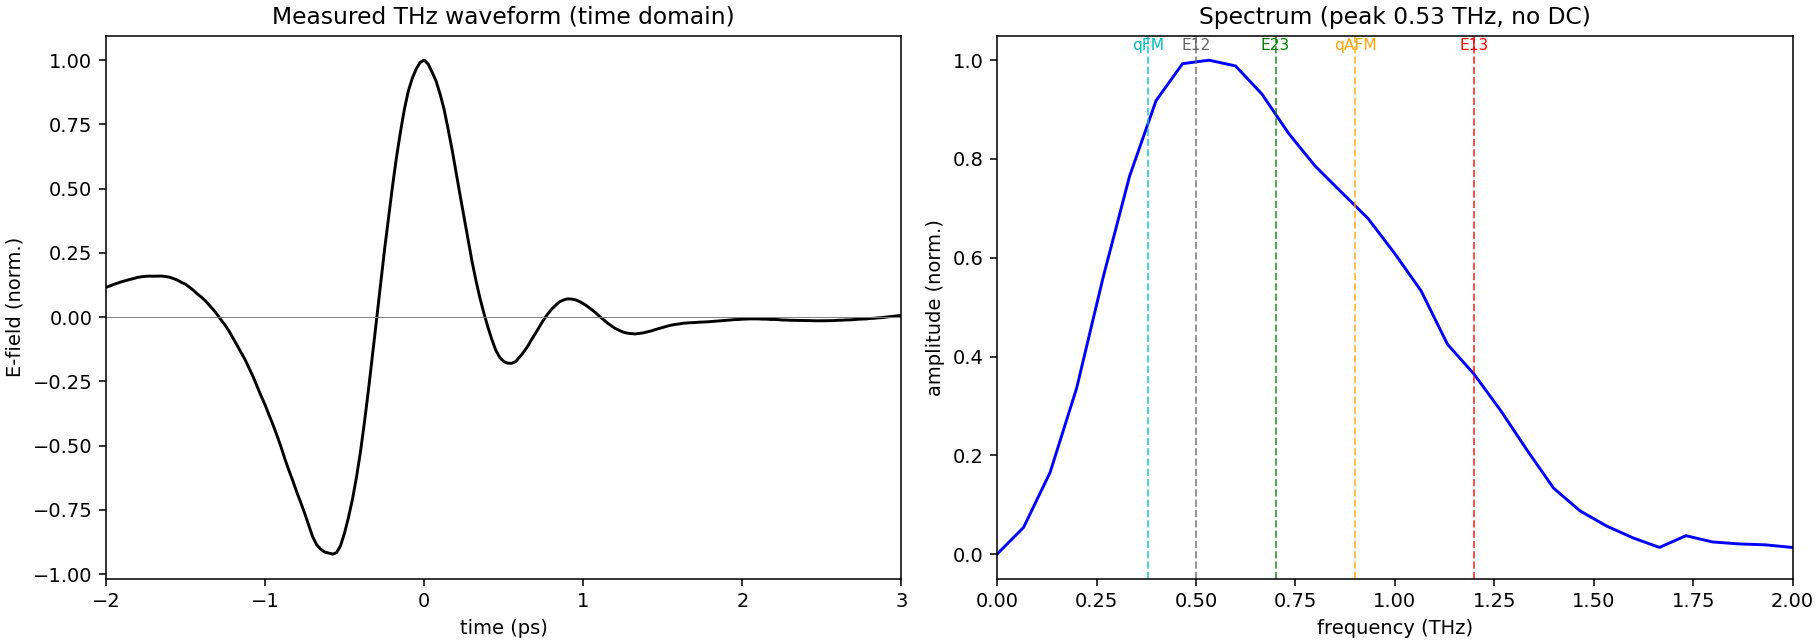
\includegraphics[width=0.95\textwidth]{../tmfeo3_2dcs_final/figures/experimental_pulse_final.png}
\caption{The measured THz pump.  Left: single bipolar cycle
($\sim1.2$\,ps, no DC).  Right: amplitude spectrum peaked at
$0.53$\,THz$\,\approx E_{12}$, covering all five modes.  The absence of
DC content removes the quasistatic-tilt legs that a Gaussian stand-in
pulse would add; the measured waveform is the cleanest configuration.}
\label{fig:si-pulse}
\end{figure}

Two consequences organize the readout physics.  First, excitation
scales as $E^2$ and detection as $E^1$ (third order).  Second, the CEF
lines are E1-bright while $\qafm$ is E1-dark but M1-bright: a magnon is
therefore read out either by borrowing a CEF electric dipole through an
Fe--Tm vertex (geometry A) or through its own magnetic dipole at the
magnon frequency (geometry B).  Using the magnetic $g$-factor instead of
$\sqrt f$ for the magnon electric emission over-weights it by
$\sim100\times$ and buries the CEF peaks under the magnon diagonal; the
oscillator-strength weighting resolves this without any tuning.

% =====================================================================
\section{Displacive verification of the $W$ mechanism}
\label{si:displacive}
% =====================================================================

The rectified two-magnon force is a suddenly switched step: its edge
carries spectral weight $\propto e^{-\omega_{12}^2\sigma^2/2}$ at the
CEF frequency, i.e.\ the $E_{12}$ quantum is drawn from the pulse
bandwidth (intra-pulse difference-frequency/impulsive-Raman), while the
magnon pair carries only the phase memory $\cos\qafm\tau$.  Verified
directly: stretching the pulse $\sigma=0.25\to1.0$ at fixed amplitude
collapses the peak by $4.5$ decades ($51.7\to1.7\times10^{-3}$), while
switching the direct Tm drive on/off changes it by $<10^{-4}$
(pure-$W$ origin).  The same sweep resolves the second Fe leg: impulsive
pulses use the resonant probe magnon (peak $\propto A^2$); longer pulses
cross over to the field-following quasistatic tilt (peak
$\propto A^1$).  The measured no-DC waveform suppresses the quasistatic
legs, which is why the experimental pulse yields the cleanest spectra.

% =====================================================================
\section{Geometry B: gate versus buildup}
\label{si:buildup}
% =====================================================================

\begin{figure}[h]
\centering
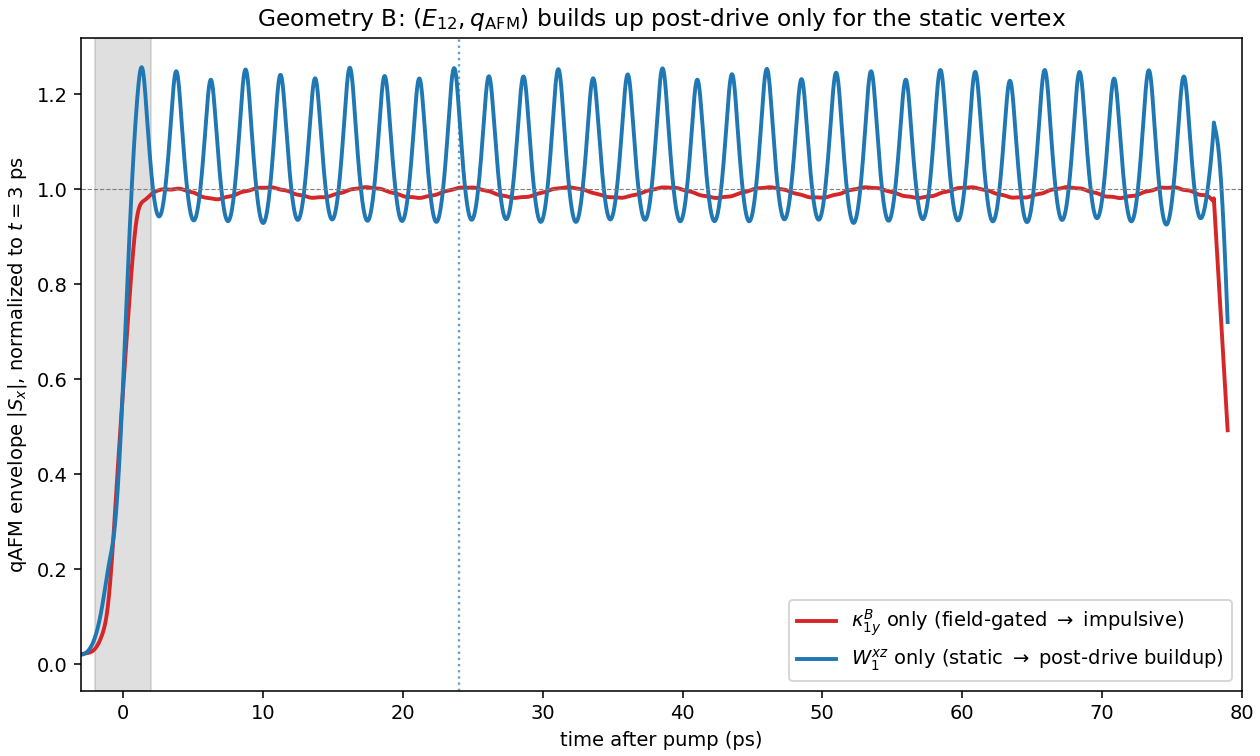
\includegraphics[width=0.7\textwidth]{../tmfeo3_2dcs_final/EXPERIMENTAL_FINAL/postdrive_buildup.png}
\caption{The $\qafm$ envelope in geometry B, normalized just after the
pump.  The field-gated $\kappa^B_{1y}$ (which alone produces the
$(E_{12},\qafm)$ cross peak) leaves a flat post-pulse envelope
(modulation $0.03$); the static $W^{xz}_1$ (which alone cannot produce
that peak) keeps exchanging the $\qfm$/$E_{12}$ reservoir with the
magnon (modulation $0.33$, envelope $\sim25\%$ above the impulsive
level).  The measured post-drive buildup requires the static vertex; the
measured transfer peak requires the gated one.}
\label{fig:si-buildup}
\end{figure}

Isolated-vertex runs: $\kappa^B_{1y}$ alone $\Rightarrow$
$(E_{12},\qafm)=0.46$ present, no buildup; $W^{xz}_1$ alone
$\Rightarrow$ peak absent, buildup present.  Both retained at $0.01$
code units.  In geometry B the Tm CEF channels $\lambda^{4\text{--}7}$
are \emph{exactly} zero (machine precision): the
$E\!\parallel\!a,H\!\parallel\!c$ drive closes on the
$\{\lambda^1,\lambda^2,\lambda^3\}$ subalgebra, an SU(2) closure that
protects geometry B from CEF contamination.

Finite temperature: $(\qfm,\qafm)$ is a pure two-magnon process and
temperature-flat; $(E_{12},\qafm)\propto n_1-n_2$ falls
$0.43\,(0\,\mathrm K)\to0.41\,(5)\to0.35\,(8)\to0.29\,(10\,\mathrm K)$.
Both peaks remain resolved through $\sim8$\,K, defining the working
window $5$--$8$\,K.

% =====================================================================
\section{The same-polarization channel: pathways, exact single-ion
verification, and the falsification ladder}
\label{si:samepol}
% =====================================================================

\subsection{Configuration}
The final same-polarization configuration (run \texttt{it14hr};
parameter files in
\texttt{tmfeo3\_2dcs\_final/params\_samepol\_final/}) is the unchanged
v4 Hamiltonian with: measured pulse; drive vector
$(0,3.0,0,0,\mathbf{0},0,0.9128,0)$ on
$(\lambda^1,\dots,\lambda^8)$---i.e.\ the $1\!\to\!3$ leg removed
($\mu^z_{13}=0$ in drive); per-leg amplitude twice the weak-probe
baseline; dampings of Table~\ref{tab:si-exp} plus population relaxation
$\gamma(\lambda^{3,8})=0.08$; Boltzmann ensemble; detection composite
$0.05\,\lambda^4+4.4\,\lambda^6$ ($\mu^z_{13}/\mu^z_{23}\approx1\%$ in
emission), magnon M1 excluded per Table~\ref{tab:si-exp}.

\subsection{Pathway assignments}
With $\mu^z_{13}=0$ the Liouville pathways of the five listed peaks are:
\begin{center}\small
\renewcommand{\arraystretch}{1.3}
\begin{tabular}{llll}
\toprule
peak $(\omega_T,\omega_t)$ & model (10\,K) & side & pathway\\
\midrule
$(+0.49,0.72)$ & $1.00$ & NR &
  $\rho_{12}\xrightarrow{\text{probe }1\leftrightarrow2}n_2(\tau\text{-phase})
  \xrightarrow{\text{probe }2\leftrightarrow3}\rho_{23}$\\
$(0.5,\,0)$ & sharpest $S_{\rm DC}$ line & --- &
  same storage, zero-frequency output leg\\
$(+0.49,1.20)$ & $0.78$ & NR &
  $\rho_{12}\xrightarrow{\text{probe }2\leftrightarrow3}\rho_{13}$,
  emission throttled by $\mu^z_{13}$\\
$(+0.91,1.18)$ & $0.20\to0.51$ ($10\to20$\,K) & NR &
  $\qafm$ delay, Fe--Tm handoff, thermally assisted\\
$(0.9,\,0.38)$ & absent & --- & carrier exists ($b$-axis M1 $\qfm$
  ridge); no $\qafm\!\to\!\qfm$ vertex\\
\midrule
$(-0.47,0.70)$ & $0.55$ & R & rephasing remnant (exact single-ion
  floor; prediction)\\
$(+0.99,0.71)$ & $0.49$ & NR & inter-site $2E_{12}$ two-quantum line
  (prediction)\\
\bottomrule
\end{tabular}
\end{center}

\subsection{Exact single-ion verification}
A standalone integrator of the 8-dimensional $\vec\lambda$ equation
(same CEF energies, dampings, measured pulse, same census pipeline;
$\sim13$\,s per 2D map versus $\sim10$\,min for the lattice) reproduces
the lattice $0.5$-family census exactly, proving the family is
single-ion physics and enabling exhaustive scans.  Two facts emerge:
(i) the rephasing/non-rephasing ratio of the $(E_{12},E_{23})$ transfer
peak has a floor of $0.47$--$0.58$ under this pulse across all drive
strengths, dipole-phase choices, and dampings---the rephasing remnant is
an exact prediction of any three-level ion driven by this waveform;
(ii) the $\omega_\tau=2E_{12}$ two-quantum line is absent in the exact
single-ion dynamics and is therefore an inter-site (mean-field) product.

\subsection{Falsification ladder}
The dark-dipole scenario was reached by exhausting the alternatives;
each row was run in the full lattice model with the blind census:
\begin{center}\small
\renewcommand{\arraystretch}{1.25}
\begin{tabular}{lll}
\toprule
hypothesis & run & outcome\\
\midrule
static mixing field $h_{\lambda^6}=0.3$ & it8 &
  over-strong: transition lines shift off calibration\\
perturbative $h_{\lambda^6}=0.06$ & it9 &
  pumps $(\qafm,E_{13})$ to $0.9$ (wrong direction); side unchanged\\
CEF detuning $0.02$\,THz (ladder break) & it10 &
  interloper survives; larger detuning barred by the observed
  degenerate lines\\
dipole triple-product sign flip & it11 & census unchanged\\
dark $\mu_{13}$ at low drive & it12 &
  population route floods the $(0,E_{23})$ band; needs the
  $2\times$ drive + $T_1$ combination\\
dark $\mu_{13}$, $2\times$ drive, $T_1$ & \textbf{it14} &
  \textbf{adopted}: both transfer peaks NR, correct hierarchy\\
negative $\mu_{13}$ leg, lower drive & it15 &
  interloper returns ($|\mu_{13}|$ acts sign-independently);
  magnon-delay family floods\\
\bottomrule
\end{tabular}
\end{center}
The $(0.9,0.38)$ peak remains the one open item: the $\qfm$ emission
carrier exists as a uniformly $\tau$-modulated $b$-axis M1 ridge in the
Fe $S_y$ channel ($\Gamma_2$ puts $\delta F_{y,z}$ at $\qfm$), but the
model lacks a $\qafm\!\to\!\qfm$ transfer vertex of sufficient
strength; one probed configuration (it15) produced a genuine
$(+0.89,0.33)$ maximum at $0.21$ relative, evidence the peak is
reachable in an extended Hamiltonian class.

% =====================================================================
\section{Data and code availability}
% =====================================================================
All parameter files, the blind-census scripts, the standalone qutrit
integrator, and the long-form derivation note
(\texttt{tmfeo3\_foundation.tex}: transported-gauge orbit formulas,
vertex diagrams, complete written-out Hamiltonian, mode inventory) are
archived with the repository
(\texttt{tfo\_project/}); every spectrum in the paper can be regenerated
from the committed \texttt{.param} files with the public
\texttt{ClassicalSpin\_Cpp} solver.

\end{document}
